\documentclass[]{report}

\usepackage{fontspec}
\setmainfont{Times New Roman}
\usepackage{indentfirst}

\usepackage[backend=bibtex,style=numeric, sorting=none]{biblatex}
\addbibresource{reference.bib}

\usepackage{graphicx}
\usepackage[margin=1.3in]{geometry}
\usepackage{algorithm}
\usepackage{algpseudocode}
\begin{document}
\begin{center}
    \Large \textbf{Milestone Report}
\end{center}

\subsection*{1.Literature Review}


In this literature review, we explore three key studies that significantly advance the field of online portfolio selection algorithms. Zhang et al.\cite*{zhang2021combining}'s first study introduces the CW-OGD strategy, a novel approach combining expert weights using online gradient descent, proving superior in terms of return, risk, and computational efficiency. Their second paper\cite*{zhang2023effective} advances the field further with a mirror gradient descent-based algorithm tailored for the long/short market, achieving dimension-free regret and enhancing performance in the Chinese futures market. Hall and Willett's\cite*{hall2015online} study shifts focus to Dynamic Mirror Descent (DMD) in online convex optimization, adept at handling high-dimensional, dynamic environments. 

Collectively, these studies represent a paradigm shift in online learning algorithms for portfolio selection, emphasizing adaptability, robustness, and efficiency, catering to the complexities of modern financial markets.

\subsection*{2.Data processing}

In our preceding research, we meticulously selected a subset of 390 stocks from the S\&P 500, each boasting a historical data span exceeding 20 years. This curated stock pool forms the foundation for testing and developing our online learning-based portfolio selection methodologies. A critical step in our process involved addressing data gaps and ensuring precise temporal alignment across all stocks. Additionally, we computed the daily returns for each stock, laying the groundwork for subsequent analysis.

As a preliminary benchmark, we established a baseline portfolio derived from our stock pool, employing a straightforward equal-weight strategy. This benchmark serves as a reference point against which the performance of portfolios curated by online learning algorithms can be evaluated. The rationale behind the equal-weight strategy is straightforward: each stock in the portfolio is assigned an identical weight, reflecting an approach of uniform distribution without bias towards any particular stock. This method provides a clear, unbiased standard for comparison, essential for assessing the efficacy of more sophisticated, algorithm-driven portfolio selection strategies.

\begin{figure}[ht]
    \centering
    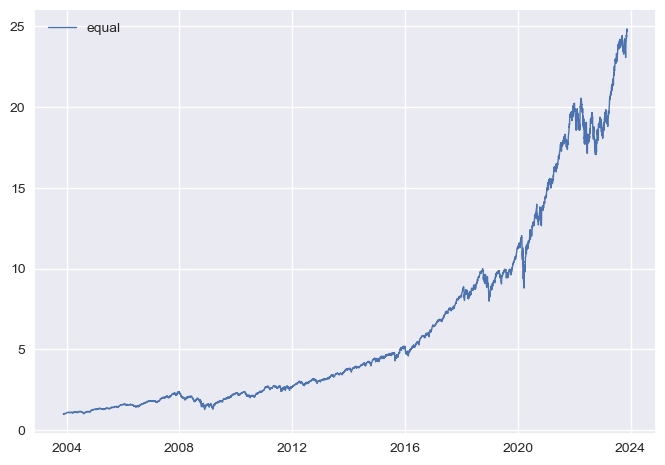
\includegraphics[width=0.8\textwidth,height=5cm]{1.png}
    \caption{equally weight portofolio}
\label{fig:euqalweight}
\end{figure}

\subsection*{3.OGD algorithm in portfolio selection}

In our OGD algorithm, we realize the daily portofolio selection and back-testing frame. At first , we set the initial weight starts from the equally weights strategy, which $x_0=\{ {1/n} \} ^n$, where n is the amount of stocks. Similarly, we define $x_t$ as the weight allocation of day $t$.
We define the matrix of return is $A_t=[r_{1,t},r_{2,t},\ldots,r_{n,t}]$. The loss function we used in OGD is linear, which represent that higher weight and higher return will generate a lower loss. Hence we can derivate the gradient $g$ in our OGD algorithm as below.
$$
L(x_t)=-A_tx_t
$$
$$
g=\nabla L(x_t)=-A
$$

OGD algorithm is operated as below.
\begin{algorithm}
    \caption[]{OGD algorithm}
    \begin{algorithmic}[1]
        \Statex \textbf{Input:} the daily return matrix $A_t$
        \Statex\textbf{Output:} the cumuative return $S_t$
        \State Initialize: Step sizes $\eta$ and weight $x_0$
        \For{$t=\{1,2,3,\ldots ,n\}$}
        \State Calculate the accumalative return until $t$ period $S_n=S_{n-1}(1+A_tx_{t-1})$
        \State Calculate the loss gradient $g=-A_t$
        \State update the portofolio $x_t= \arg \min_{x\in \textbf{X}}\langle\eta g,x \rangle+\frac{1}{2}||x_{t-1}-x||$
        \EndFor
        
    \end{algorithmic}
\end{algorithm} 


OGD algorithm performs better than the benchmark strategy. However, we found that the volitility of OGD portfolio is much higher than the equally weight strategy. In spite of that, it has a better result in the accumulative return perspective. We will keep on improving our model in the future.

\begin{figure}[ht]
    \centering
    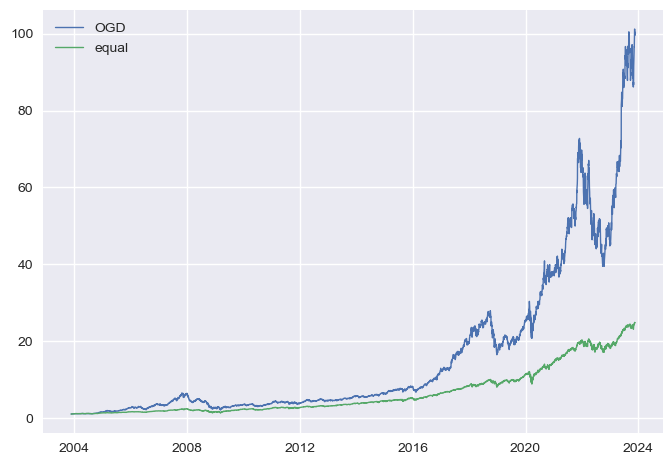
\includegraphics[height=5cm,keepaspectratio]{2.png}
    \caption{equally weight portofolio}
\label{fig:euqalweight}
\end{figure}
\subsection*{4.Future plan}
In the next phase, we will implement and test the OMD, RM, RM+ algorithms for portfolio construction, following the successful application of OGD. On the same time, We will improve the step size $\eta$ and the loss function. We will consider a method that could help us include the risk in the portfolio selection by designing new loss function on sharpe ratio or similar concepts. Based on OGD, we found that it is quiet slow when it adjusted its portfolio although step size $\eta$ is a relatively large number. We will try to make $\eta$ auto-adaptive in the dynamic market.

For the second phase of our future plan, we will introduce a novel mixed-weight strategy, leveraging a two-tiered online learning approach. This strategy will dynamically combine the strengths of different algorithms we have tested, including OGD, OMD, RM, and RM+.  This approach represents a significant advancement in adaptive portfolio management, ensuring a more resilient and responsive strategy in the face of financial market uncertainties.
hi
\printbibliography

\end{document}